\section{Objectifs}

Les objectifs de ce second hands-on sont:

\begin{itemize}
    \item[-] D'utiliser le matériel mis à disposition (i.g. oscilloscope, multimètre, etc ...) afin de vérifier les composants et les signaux d'intérêt
	\item[-] De comprendre l'utilité d'un comparateur dans ce contexte
	\item[-] De pouvoir définir un tension de référence à l'aide d'un diviseur résistif 
	\item[-] De se familiariser avec le NE555 et son utilisation en mode bascule monostable
	
\end{itemize}

\begin{figure}[!ht]
	\centering
	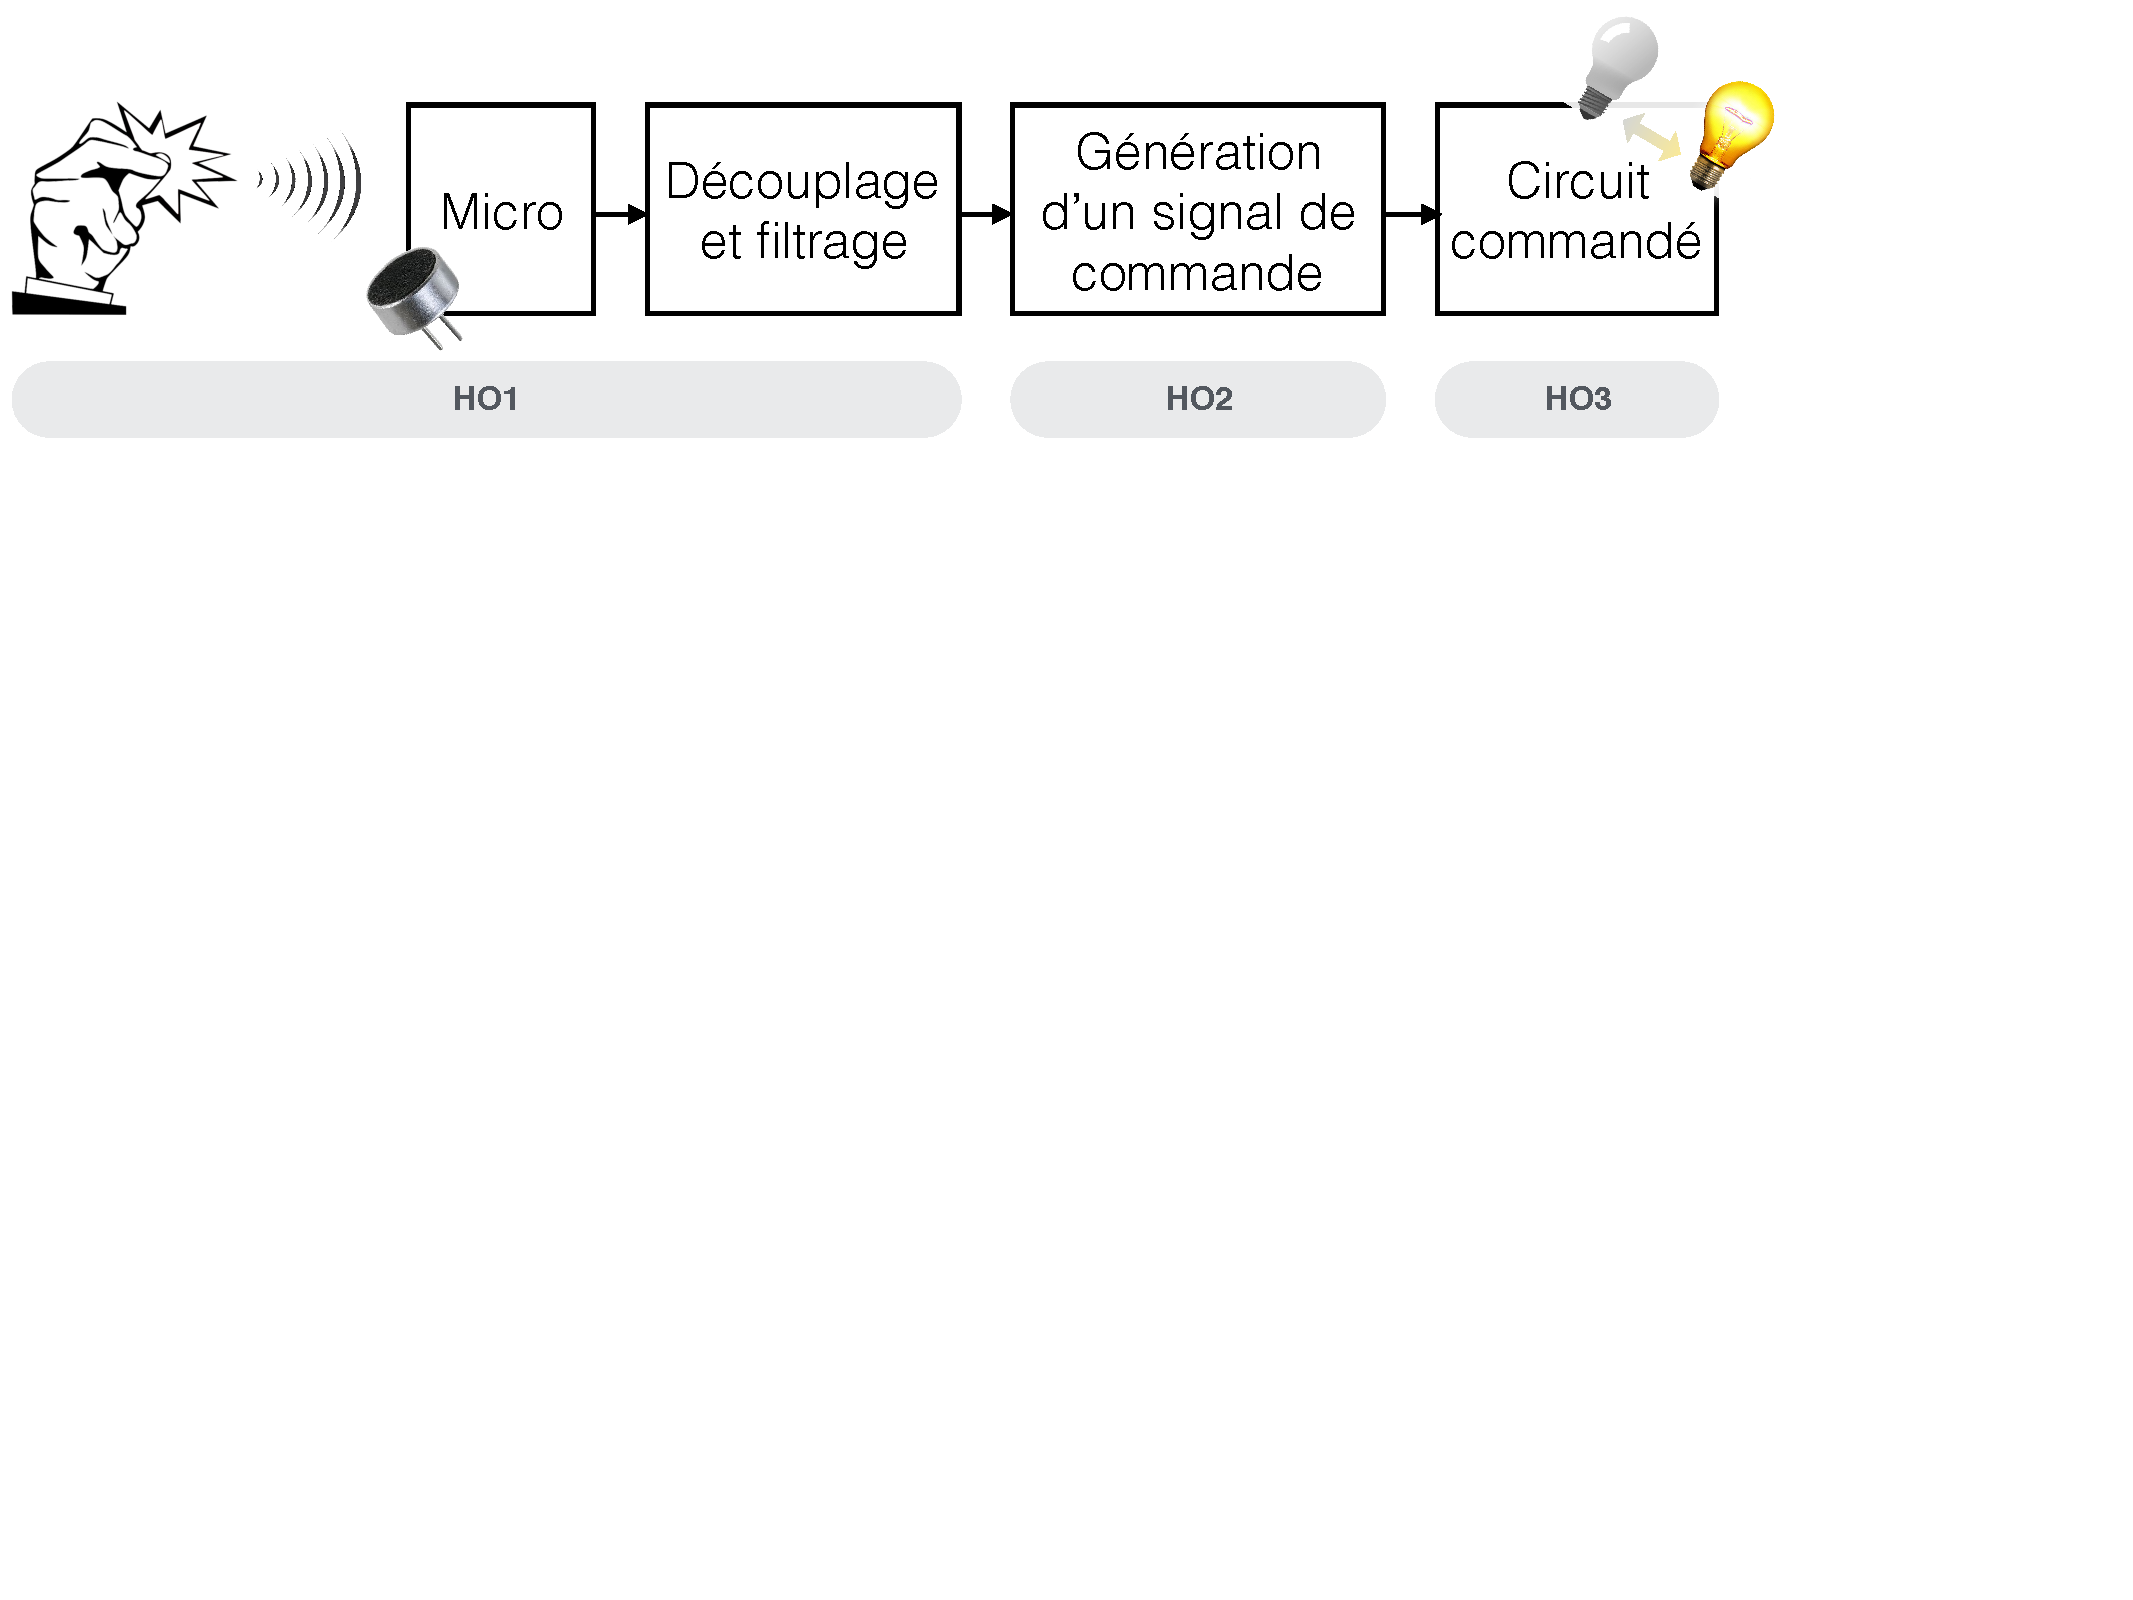
\includegraphics[width=0.9\textwidth]{figures/SchemaBloc.pdf}
	\caption{Schéma-bloc du circuit.}
	\label{fig:block-diagram}
\end{figure}

Le schéma-bloc du circuit est présenté à la Figure \ref{fig:block-diagram}. La génération d'un signal de commande propre est cruciale dans ce circuit: il s'agit en quelques sortes de l'interface entre d'une part, le signal obtenu au moyen du capteur et d'autre part le signal de type ON/OFF qui sert à modifier l'état du système commandé. 